\chapter{Bisherige Forschung und Theorie}
\label{ch:bisherige-forschung}

Um die notwendige Basis für die vorliegende Arbeit zu schaffen, wird zunächst ein Blick auf die bisherige Literatur geworfen.
Beginnend mit einem allgemeinen Blick auf kognitive Verzerrungen als Teil der psychologisch-kognitiven Forschung, ihren Ursachen sowie Beispielen der genannten Phänomene liegt der Fokus insbesondere auf impliziten Stereotypen.
Als Möglichkeit, die Auswirkungen des implicit bias zu reduzieren wird anschließend eine Einführung zur Thematik der Bias Awareness geliefert sowie bisherige Literatur dazu überprüft.
Anschließend wird diskutiert, inwiefern Biases im schulischen Kontext präsent sind und in welchen Aspekten sich ihre Auswirkungen auf das Lehren und Lernen äußern.
Schließlich wird darauf eingegangen, welche Einflüsse die Itemformulierung bei Fragebögen auf die Erfassung der Bias Awareness hat.


\section{Kognitive Verzerrungen}
\label{sec:kognitive-verzerrungen}

Unter kognitiven Verzerrungen (englisch: \emph{cognitive biases} oder \emph{cognitive illusions}) versteht man psychologische Effekte, welche zu einer Wahrnehmung oder Beurteilung führen, die von der realen Situation abweicht \citep{pohl2004cognitive}.
Die zahlreichen Manifestationen dieser Verzerrungen äußern sich auf verschiedene Art und Weise -- einen Überblick liefert \autoref{fig:cognitive-bias-cheat-sheet}.

\begin{figure}[h!]
	\centering
	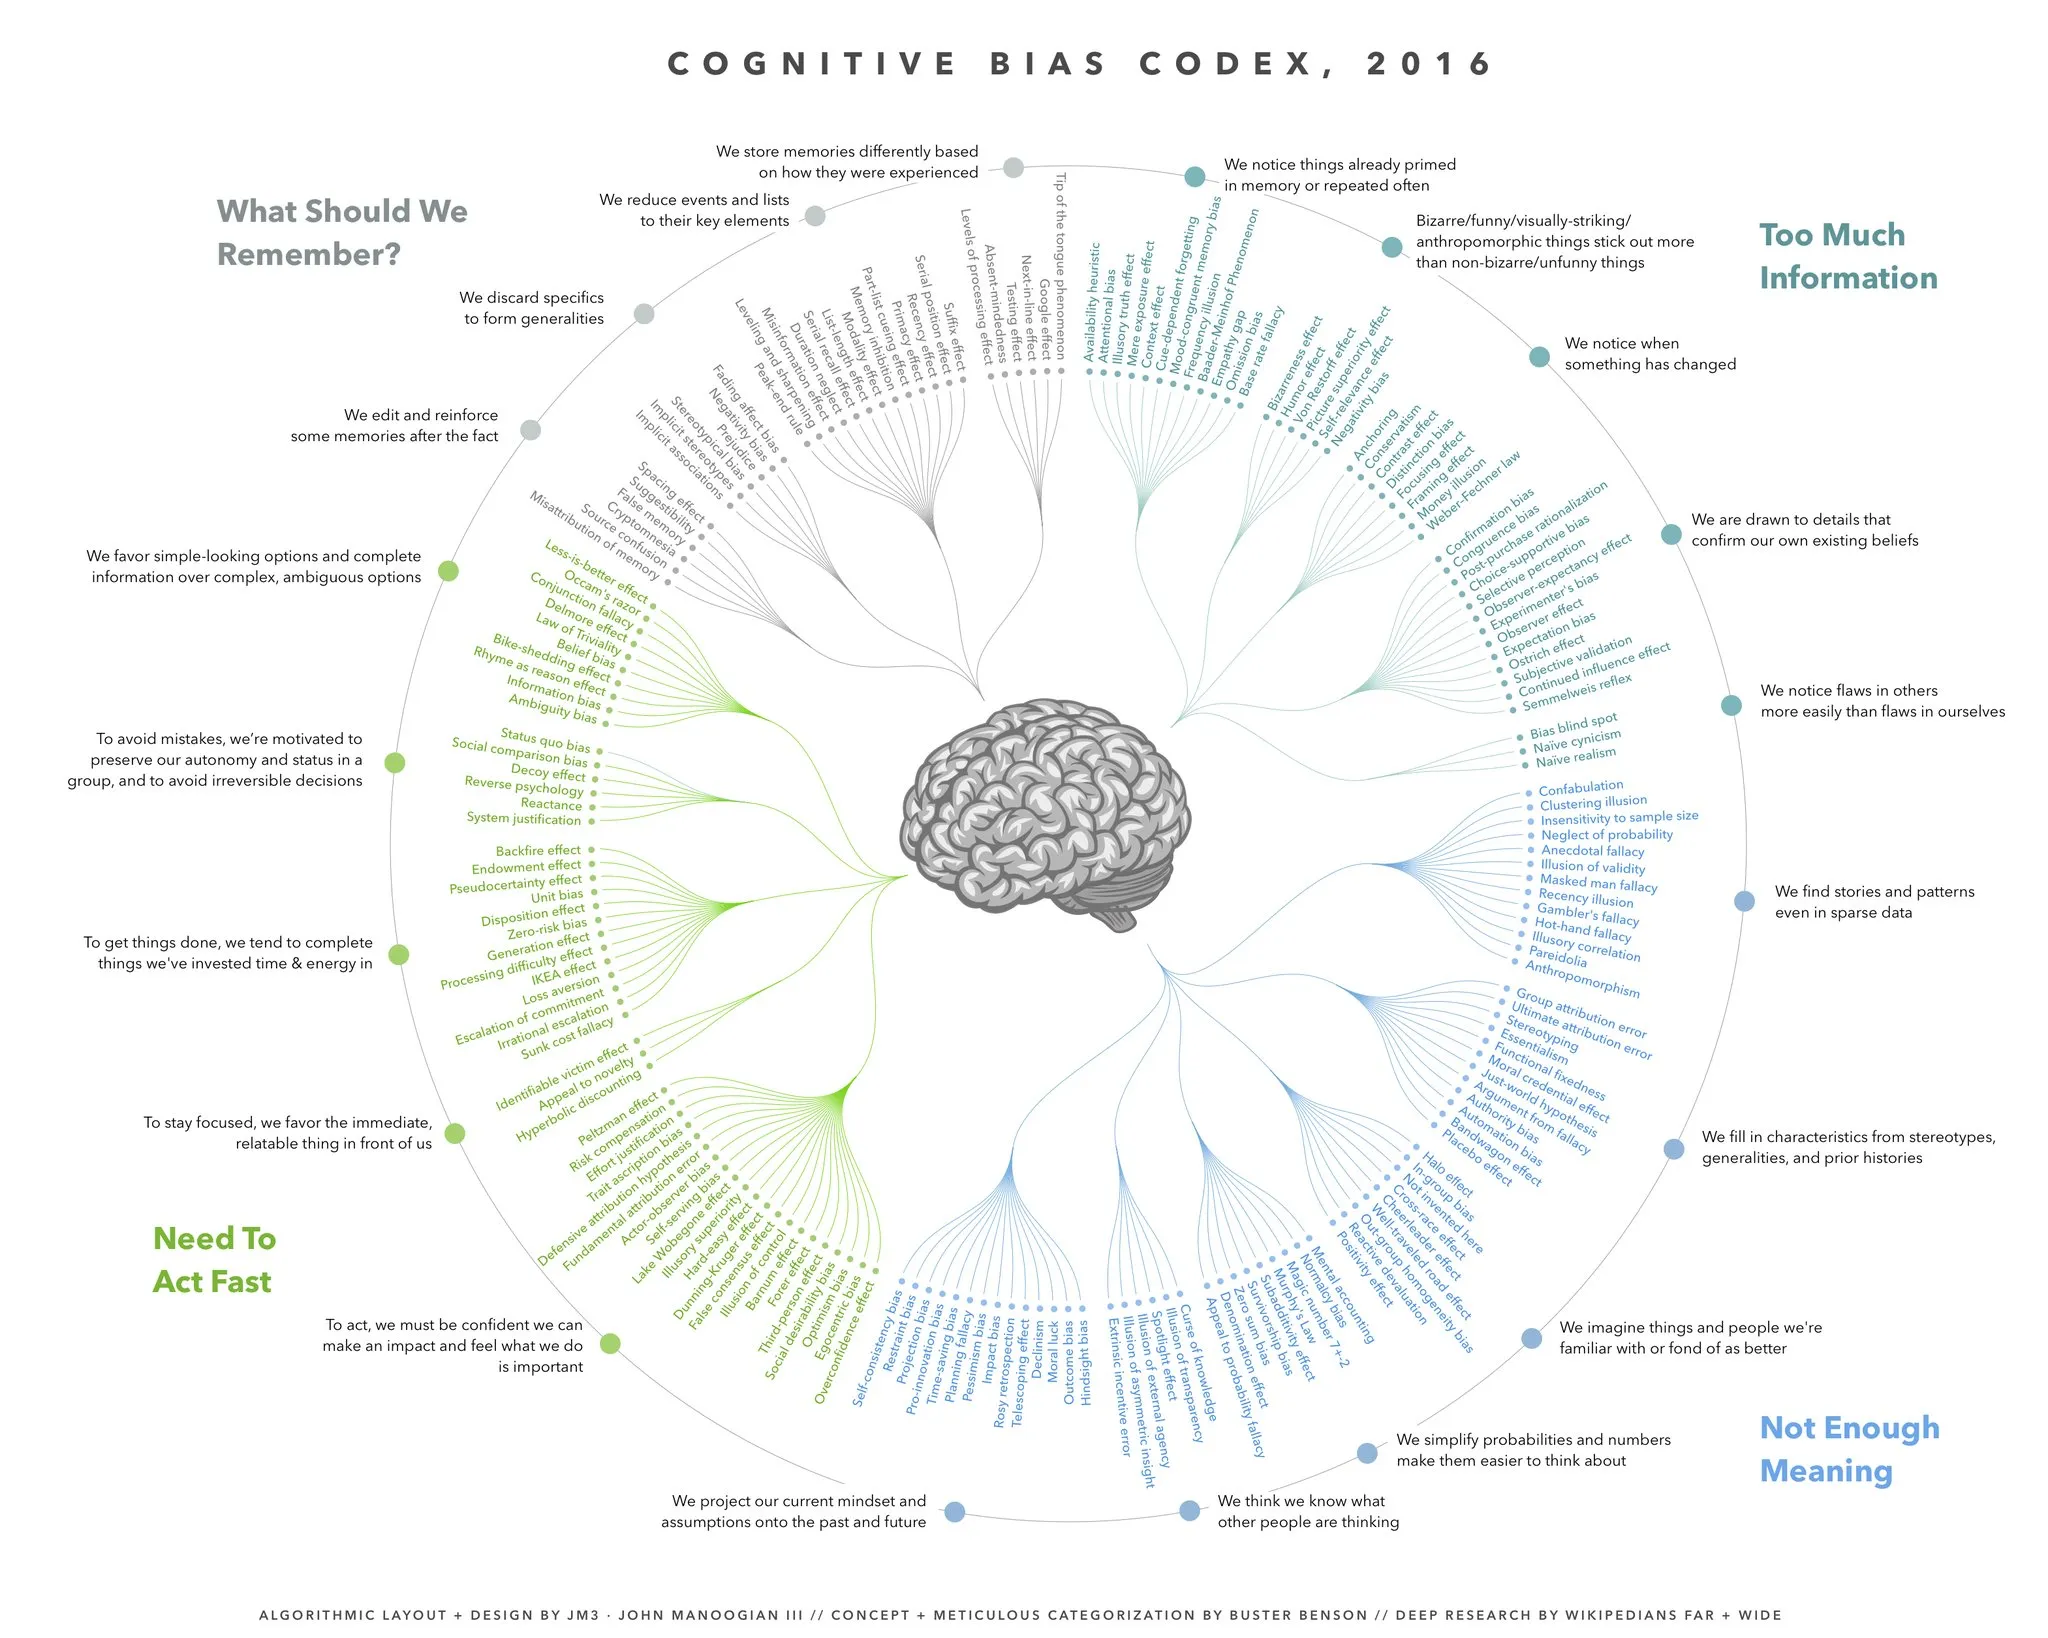
\includegraphics[width=\textwidth]{resources/cognitive-bias-cheat-sheet.png}
	\caption[Cognitive Bias Codex]{Cognitive Bias Codex -- Beispiele verschiedener kognitiver Biases \citep{benson2016cognitive}}
	\label{fig:cognitive-bias-cheat-sheet}
\end{figure}

Wie in \autoref{fig:informationskreislauf} dargestellt werden bei der Integration neuer Informationen vier Phasen durchlaufen.
Aus der riesigen Menge der auf uns einströmenden Informationen werden zunächst einige wenige selektiert, aus welchen wir uns mithilfe unserer bisherigen Erinnerung einen Sinn machen können.
Unser Vorwissen wird dann genutzt, um sie in einen Kontext einzubetten, welcher anschließend unser Handeln beeinflusst.
Diese Handlungen fließen danach wiederum in unsere Erinnerung ein, auf die bei neuen Informationen zugegriffen wird.

\begin{figure}[h!]
	\centering
	\includegraphics[width=0.5\textwidth]{resources/informationskreislauf.jpg}
	\caption{Kreislauf der Integration von neuen Informationen}
	\label{fig:informationskreislauf}
\end{figure}

Bei jedem Phasenübergang finden dabei Filtereffekte statt.
Nach \cite{benson2016cognitive} kristallisieren sich dabei vier Problemstellungen heraus, mit denen das menschliche Gehirn tagtäglich konfrontiert wird.
Jede der folgenden Kategorien repräsentiert dabei einen der dargestellten Übergänge zwischen den Phasen.

\begin{enumerate}
	\item \emph{Informationsüberflutung}: Bereits seit Beginn der Existenz menschlicher Aufzeichnungen von Informationen existiert das Problem der Überflutung durch ebenjene \citep{bawden2020information}.
	Aufgrund technischer Entwicklungen und der Verbreitung des Internets hat sich die Menge an Informationen, die auf uns einwirken, insbesondere in den letzten Jahrzehnten extrem vergrößert \citep{siegler2010every}.
	So gaben 22.5\% der Deutschen im Jahr 2021 Informationsüberflutung als eine der Hauptursachen für Stress an \citep{meyer2021entspann}.
	Dies beeinflusst auch die Qualität professioneller Entscheidungen, beispielsweise im Gesundheitssystem \citep{hall2004information}, beim Management von Personal \citep{volnhals2008information} und Marketing \citep{meyer1998information} oder in der Wissenschaft \citep{landhuis2016scientific}.
	
	Nach der \emph{cognitive load theory} \citep{atkinson1968human} ist das menschliche Arbeitsgedächtnis sehr begrenzt.
	Aufgrund der übermächtigen Menge an Informationen, die auf uns einwirken, sind unsere Gehirne daher dazu gezwungen, aggressiv zu filtern \citep{savolainen2007filtering}.
	Das Resultat können fehlerhafte Schlussfolgerungen sein, beispielsweise in Form eines \emph{confirmation bias} \citep{goette2019information}.
	
	\item \emph{Mangel an Kontext}: Die Welt, in der wir leben, ist sehr komplex.
	Dennoch ist es notwendig, dass wir aus den wenigen uns gegebenen Informationen korrekte Vorhersagen treffen und ihnen eine angemessene Bedeutung zuweisen.
	Das Erkennen von Mustern trotz eines Mangels an Kontext ist in der Realität häufig unausweichlich.
	Doch gerade deshalb kann es vorkommen, dass wir eine Übergeneralisierung vornehmen und Beziehungen zwischen Informationen herstellen, obwohl diese nicht oder anders existieren.
	
	Ein Beispiel dafür ist die sogenannte \emph{Konfabulation} \citep{gilboa2002cognitive}:
	Eine Person meint, sich an ein Ereignis zu erinnern und kann konkrete Erinnerungen dazu nennen -- jedoch stellen sich diese bei Überprüfung als falsch bzw. ausgedacht heraus.
	Bekannt ist diese Art der kognitiven Verzerrung z.B. durch den \emph{Mandela-Effekt}, eine kollektive Konfabulation, nach der Nelson Mandela bereits in den 1980er-Jahren in Haft (und nicht erst 2013 in Freiheit) gestorben sei.
	Ein ähnlicher Effekt kann auch in Bezug auf visuelle Erinnerungen beobachtet werden \citep{prasad2022visual}, beispielsweise erinnern sich viele Menschen an einen Monopoly-Mann mit Monokel, obwohl dieser nie mit Monokel dargestellt worden ist.
	
	%TODO: Eventuell diesen Teil hinter die Aufzählung verschieben? Unterscheidung explicit/implicit stereotype
	Besonders relevant für diese Arbeit ist auch die Bildung von \emph{Stereotypen}.
	Dabei handelt es sich um ``weitverbreitete, jedoch feste und stark vereinfachte Bilder oder Vorstellungen zu einem bestimmten Typ von Personen oder Dingen'' \citep[Übers. d. Verf.]{bordalo2016stereotypes}.
	Insbesondere in Bezug auf die Zugehörigkeit zu ethnischen Gruppen \citep{brigham1971ethnic, guichard1977ethnic, mastro2009effects} und Geschlecht \citep{hoffman1990gender, heilman2012gender, haines2016times, ellemers2018gender} gab und gibt es immer noch viel aktuelle Forschung, die sich mit den (insbesondere negativen) Auswirkungen von Stereotypen befasst.
	
	\item \emph{Notwendigkeit, schnell zu handeln}: Trotz der Fülle an Informationen, die auf uns einströmen, dürfen wir uns nicht durch das Abwägen von Optionen aufhalten lassen, sondern müssen zuverlässig schnelle und gute Entscheidungen treffen.
	Aus diesem Grund liegt unser Fokus häufig auf den offensichtlichen und einfachen Dingen, anstatt sich in den komplizierten Details der Situation zu verlieren.
	Ein Beispiel hierfür ist der \emph{identifiable victim effect}, nach dem Menschen eher bereit sind, Ressourcen für konkrete und identifizierbare als für abstrakte, statistische Opfer bereitzustellen \citep{jenni1997explaining}.
	Weiterhin beschäftigen wir uns eher mit Trivialiäten als komplexen Problemen \citep{parkinson1958parkinson}, wie der \emph{bike shed effect} visualisiert:
	Je weniger komplex das Problem, desto mehr Zeit wird dafür aufgewendet, eine Entscheidung darüber zu treffen.
	
	Damit wir trotz des Informationsmangels nicht zögern zu handeln, überschätzen wir unsere Fähigkeiten und Urteilskraft häufig (\emph{overconfidence effect}, \cite{moore2008trouble}) und legen höheren Wert auf unsere eigene Wahrnehmung \citep{ross1979egocentric}.
	Diese Überschätzung findet insbesondere dann statt, wenn unsere tatsächliche Kompetenz relativ niedrig ist, wie der bekannte \emph{Dunning-Kruger-Effekt} \citep{dunning2011dunning} zeigt.
	
	\item \emph{Fehlbarkeit von Erinnerungen}: Nachdem wir der Informationsflut mit radikaler Filterung und Selektion begegnet sind, ihr vermeintlichen Kontext zugewiesen haben und auf Basis dieser Entscheidungen gehandelt haben, stehen wir vor einem weiteren Problem.
	Über die Nützlichkeit dieser Informationen in der Zukunft muss spekuliert werden, und so kommt es zu Verzerrungen der Realität.
	Liegt eine Liste von Informationen vor, spielt beispielsweise die Position innerhalb dieser eine große Rolle für die Erinnerung \citep{murdock1962serial, phillips1967effects}.
	
	Dass unsere Erfahrungen beeinflussen, wie wir uns an Dinge erinnern, zeigt sich unter Anderem beim \emph{self-reference effect} \citep{rogers1977self}.
	Hierbei sind Erinnerungen an Informationen, die uns nicht persönlich betreffen, deutlich weniger zuverlässig als jene, die eine hohe persönliche Relevanz haben.
	Auch der sogenannte \emph{google effect} \citep{sparrow2011google} spiegelt wider, dass unsere Erinnerung abhängig von der Situation ist:
	Im Wissen, dass die betreffende Information durch eine kurze Internetrecherche schnell wieder abrufbar ist, 
	sehen wir nur eine reduzierte Notwendigkeit, sich insbesondere an spezielle Details zu erinnern.
\end{enumerate}


\section{Implizite Stereotypen}
\label{sec:implicit-bias}

Beim \emph{impliziten Stereotyp} (oder auch \emph{implicit bias}) handelt es sich um ``eine Reihe von Überzeugungen über Merkmale, welche für die Mitglieder einer sozialen Kategorie charakteristisch sind'' \citep[Übers. d. Verf.]{greenwald1995implicit}.

Wie schon durch den Namen angedeutet, handelt es sich hierbei um ein Teilgebiet der Stereotypen, welche schon in \autoref{sec:kognitive-verzerrungen} angesprochen wurden.
Um die Bedeutung des Begriffs abzugrenzen ist es essenziell hinzuzufügen, dass es sich beim implicit bias um unbewusste Einflüsse auf das Denken handelt.
Die ebenfalls gebräuchliche Bezeichnung des \emph{explicit stereotype} stellt im Gegensatz dazu aktive und bewusste Einstellungen dar.

Eine weitere wichtige Unterscheidung muss zwischen Stereotypen und Vorurteilen gemacht werden.
Während es sich beim sozialpsychologischen Begriff des Stereotyps um kognitive Zuordnungen zu einer bestimmten sozialen Kategorie handelt, bezeichnet das Vorurteil die subjektive Bewertung und emotionale Reaktion \citep{degner2022vorurteile}.
Bei beiden Begriffen handelt es sich jedoch um Konzepte, welche die Einstellungen zu Menschen bestimmter sozialer Gruppen unabhängig von deren individuellen Eigenschaften widerspiegeln.

Die Bildung von Stereotypen und deren Anwendung im Alltag findet bereits im Kindesalter statt \citep{martiny2020theoretischer}.
Schon bei Kleinkindern im Alter von wenigen Monaten findet eine Identifizierung charakteristischer sozialer Eigenschaften statt \citep{killen2013children}.
Dies geschieht im Rahmen sozialer Kategorisierung, bei welcher es sich um eine Vorstufe zur Stereotypenbildung handelt.
Hierbei werden Menschen mit einer oder mehreren Gemeinsamkeiten zu einer sozialen Gruppe zusammengefasst.
Die Einordnung von Objekten und Menschen in Kategorien ist ein Prozess, der regelmäßig und weitgehend automatisch stattfindet \citep{macrae2000social}.
Diese Gruppierung hilft dabei, die Komplexität sozialer und so die damit einhergehende kognitive Belastung zu reduzieren sowie leichtere Vorhersagen zu treffen \citep{killen2013children}.
Beispielsweise ist die Erinnerung von Kindern an Informationen, welche ihrem kognitivem Schema entsprechen, stärker als wenn dies nicht der Fall ist \citep{bigler1993cognitive}.

Beobachten lassen sich die Effekte dieser Kategorisierung ebenfalls bereits im frühen Kindesalter:
So zeigen schon drei Monate alte Säuglinge Präferenzen gegenüber den Gesichtern von Mitgliedern der eigenen Ethnie gegenüber denen von Mitgliedern anderer Ethnien \citep{kelly2005three}.
Das Vorhandensein impliziter Stereotype ließ sich ab einem Alter von 4--9 Jahren zeigen \citep{bigler1993cognitive}, während explizite Vorurteile ebenfalls ab einem Alter von 4 Jahren gebildet werden \citep{aboud1993developmental}.
Es wird davon ausgegangen, dass viele Stereotype erlernt sind und stark durch das soziale Umfeld geprägt werden.
Kinder nutzen dabei den Vergleich mit Beispielen \citep{martin1981schematic} und Gegenbeispielen \citep{slaby1975development}, um die eigene Gruppenzugehörigkeit abzugrenzen und erwartetes Verhalten vorherzusagen \citep{tajfel1979integrative}.

Nach dem \emph{Stereotype Content Model} \citep{fiske2002model} lassen sich Stereotype anhand der zwei Dimensionen \emph{Wärme} und \emph{Kompetenz} kategorisieren.
Während die Dimension der Wärme beschreibt, ob die betreffende Gruppe als freundlich oder feindlich gesinnt wahrgenommen wird, stellt die Dimension der Kompetenz den zugewiesenen sozialen Status dar.
Wie in \autoref{tab:implicit-stereotype-warmth-competence} dargestellt, werden je nach Wärme und Kompetenz unterschiedliche Emotionen bzw. Vorurteile mit den Stereotypen verbunden \citep{cuddy2008warmth}.
So werden beispielsweise arme Menschen, welche selbst einen niedrigen sozio-ökonomischen Status haben, jedoch gleichzeitig als Bedrohung für den eigenen Status wahrgenommen werden, häufig mit der Emotion Verachtung in Verbindung gebracht.

\begin{table}[h!]
	\begin{tabularx}{\textwidth}[h]{cc|>{\centering\arraybackslash}X|>{\centering\arraybackslash}X}
		&& \multicolumn{2}{c}{\textbf{Kompetenz}}\\
		&& niedrig & hoch\\
		\hline
		\multirow{4}{*}{\rotatebox[origin=c]{90}{\textbf{Wärme}}} & \multirow{2}{*}{\rotatebox[origin=c]{90}{hoch}} & Mitleid & Bewunderung\\
		&& z.B. ältere Menschen & z.B. Freunde\\
		\cline{2-4}
		& \multirow{2}{*}{\rotatebox[origin=c]{90}{niedrig}} &  Verachtung & Neid\\
		&& z.B. arme Menschen & z.B. reiche Menschen
	\end{tabularx}
	\caption[Stereotype Content Model]{Stereotype Content Model (Darstellung nach \cite{fiske2002model})}
	\label{tab:implicit-stereotype-warmth-competence}
\end{table}

Auch wenn die Bildung von Stereotypen ein universell stattfindender Prozess ist, der grundsätzlich viele Vorteile mit sich bringt, lassen sich viele negative Effekte darauf zurückführen.
Beispielsweise führen stereotypisierte Gruppen negatives Feedback eher auf Stereotype zurück, während positives Feedback eher als Mitleid interpretiert wird \citep{crocker1991social}.
Weiterhin können implizite Stereotype zu selbsterfüllenden Prophezeihungen führen \citep{latu2015gender}.
Zum Beispiel kann ein Arbeitgeber, der ein negatives Bild von Frauen in Führungspositionen hat, diese in Bewerbungsgesprächen durch seine Rückmeldungen negativ beeinflussen und somit zu einem schlechteren Ergebnis der Bewerberin führen.
Zusätzlich können bekannte Stereotype das Selbstbild von Mitgliedern der betroffenen Personengruppe negativ beeinflussen \citep{cox2012stereotypes, ebert2013positionsartikel}.
Dies kann zu einer Internalisierung der mit dem Stereotyp verbundenen Eigenschaften führen.
Die Angst von Betroffenen, aufgrund von Stereotypen zu beurteilt zu werden oder existierende Vorurteile durch ihr Verhalten zu bestätigen, ist ein häufiges Phänomen, was unter dem Namen \emph{stereotype threat} bekannt ist \citep{steele1995stereotype, keller2003stereotype}.
Der Effekt der selbsterfüllenden Prophezeihung akkumuliert sich außerdem \citep{madon2018accumulation}, d.h. je mehr Menschen stereotypische Erwartungen haben, desto größer die Reaktion im Verhalten der betroffenen Person.

Stereotype und Vorurteile sind häufig die Ursache offener Diskriminierung.
Beispielsweise lässt sich die Diskriminierung von bestimmten Gruppen bei Jobinterviews auf die Stereotypisierung zurückführen -- ein Effekt, der sich bei übergewichtigen Menschen \citep{agerstrom2011role}, Homosexuellen \citep{tilcsik2011pride} sowie weiblichen Bewerberinnen \citep{picho2013exploring, latu2015gender} beobachten lässt.


\section{Bias Awareness}
\label{sec:bias-awareness}

Wie bereits in \autoref{sec:implicit-bias} beschrieben handelt es sich beim implicit bias um kognitive Verzerrungen, über deren Existenz sich das Individuum nicht bewusst ist.
In Studien konnte jedoch gezeigt werden, dass Vorurteile nach einer Intervention, welche über deren Vorhandensein aufklärt, wesentlich geringer ausfallen \citep{penner1970interpersonal, grube1994inducing}.
Auch neuere Studien konnten bestätigen, dass sich Menschen weniger diskriminierend verhalten oder die negativen Effekte ihrer Vorurteile kompensieren, wenn ihnen diese bewusst gemacht werden \citep{monteith1993self, monteith2010aself, monteith2010bself, pope2018awareness}.
\textciteauthor{rohner2013reducing} konnten außerdem demonstrieren, dass der attractiveness bias bei Bewerbungsgesprächen reduziert werden kann, wenn die Versuchspersonen vor der Bewertung der Bewerbungen über die Existenz des Bias aufgeklärt wurden und das Ausmaß ihres eigenen Bias einschätzen mussten.
Dieser Effekt trat nicht auf, wenn lediglich eine Aufklärung stattfand.
Dies spricht dafür, dass erst die aktive Einschätzung der kognitiven Verzerrungen (eventuell durch eine damit verbundene Erhöhung der Bias Awareness) zur Reduzierung der negativen Auswirkungen führt.

Der Grad, zu welchem sich ein Individuum über die eigenen implicit biases bewusst ist, wird nach \citet{perry2015modern} als \emph{bias awareness} bezeichnet.
Zusätzlich zu einer Reduktion der Auswirkungen des implicit bias konnten \textciteauthor{perry2015modern} zeigen, dass eine höhere Bias Awareness dabei helfen kann, den Einfluss von Biases auf beobachtete Handlungen zu erkennen.

Doch warum reduzieren sich die Effekte der Vorurteile beim Bewusstwerden über deren Existenz?
Nach der \emph{Belief System Theory} \citep{rokeach1968theory, grube1994inducing} leben Menschen nach einer Menge an Werten, die ein zusammenhängendes System bilden.
Ihre Handlungen und ihr Denken richten die Personen nach diesen Wertevorstellungen aus und nutzen diese, um ihr Handeln als gut oder schlecht zu bewerten.
In manchen Situationen -- beispielsweise nach der Aufklärung über Vorurteile -- werden wir nun damit konfrontiert, dass unser Verhalten nicht im Einklang mit unserem Wertesystem steht.
Diese Differenz führt dazu, dass wir zukünftig in ähnlichen Situationen stärker darauf achten, unsere Handlungen an unseren Werten auszurichten.

Nach \citet{perry2015modern} gibt es trotz der generellen Tendenz, dass eine höhere Bias Awareness das Ausmaß von Vorurteilen sowie deren Effekte reduzieren kann, starke individuelle Unterschiede.
So existieren beispielsweise Differenzen in der individuellen Motivation, sich frei von Vorurteilen zu verhalten \citep{devine2002regulation, plant1998internal}.
Zusätzlich erkennen manche Personen auch nicht, dass ihr Verhalten ihren Werten widerspricht \citep{monteith1998proneness} oder reagieren sich bei Konfrontation defensiv.
Doch auch nach dem Erkennen der eigenen Vorurteile existieren Unterschiede im Ausmaß, zu dem die daraus resultierenden negativen Effekte ausgeglichen werden können \citep{moskowitz2011egalitarian}.


\section{Implicit Bias und Bias Awareness im schulischen Kontext}
\label{sec:biases-schule}

Es gibt zahlreiche Gründe dafür, dass auch heute noch viele Differenzen in Bezug auf schulischen Erfolg im deutschen Schulsystem bestehen.
Im IQB-Bildungstrend 2021 konnten sowohl geschlechtsbezogene, soziale als auch zuwanderungsbezogene Disparitäten festgestellt werden \citep{iqb2021bildungstrend}.
%TODO: PISA-Studie 2018 vielleicht hier reinfließen lassen? Was sind die Ergebnisse?

Die Erwartungen der Lehrkräfte haben einen signifikanten Einfluss auf die schulischen Erfolge sowie die Motivation der unterrichteten Kinder \citep{gentrup2020self}.
Auch die impliziten Stereotype der Lehrkräfte spielen dabei eine Rolle für die Entwicklung von Unterschieden in Bezug auf Leistung und Motivation der Schülerinnen und Schüler.
Beispielsweise werden Kinder mit türkischem Migrationshintergrund und Jungen im Fach Deutsch bei gleichen Ergebnissen wie die Vergleichsgruppe schlechter bewertet, während Kinder mit osteuropäischem Migrationshintergrund oder mit höherem sozio-ökonomischen Status im Fach Mathematik bei gleichen Leistungen besser bewertet werden \citep{lorenz2016stereotype}.
Zahlreiche Studien konnten die Existenz und Auswirkungen sowohl geschlechtsbezogener \citep{keller2003stereotype, hermann2020maedchen, muntoni2020geschlechterstereotype}, ethnischer \citep{steele1995stereotype, glock2015preservice, glock2017bad, glock2019studies, costa2023does} als auch sozioökomomischer Stereotype \citep{tobisch2017negatively, kleen2020sag} im schulischen Kontext feststellen.

\textciteauthor{martiny2020theoretischer} argumentieren, dass nicht nur die negativere Bewertung durch biasbeeinflusste Lehrkräfte einen negativen Effekt auf den schulischen Erfolg der betroffenen Schülerinnen und Schüler hat, sondern auch das Gruppenzugehörigkeitsgefühl leidet \citep{martiny2020theoretischer}.
Infolge des stereotype threats können Stereotype den betroffenen Personen das Gefühl geben, nur als Repräsentant ihrer Gruppe und nicht als Individuum gesehen zu werden und infolgedessen die wahrgenommene Eingebundenheit in der Klasse reduzieren \citep{walton2012social}.
Dies wiederum kann sich negativ auf die Motivation und die Leistungen der Schülerinnen und Schüler auswirken.

Auch die Identifikation mit der Domäne, also beispielsweise dem akademischen Bereich an sich, leidet darunter, wenn die Zugehörigkeit zu einer bestimmmten sozialen Gruppe stereotypisiert ist \citep{crocker1989social}.
Nach \citet{osborne2011identification} geht eine höhere Domänenidentifikation mit dem Bildungsbereich jedoch häufig mit besseren akademischen Leistungen einher, was weitere negative Effekte für stereotypisierte Personen nach sich zieht.

Zusätzlich zu den negativen Auswirkungen für Schülerinnen und Schüler durch implizite Stereotypen konnte auch gezeigt werden, dass implicit biases in Bezug auf ethnische Hintergründe zum Risiko für Burnout der Lehrkraft beitragen können \citep{costa2023does}.

Es gilt also, den implicit bias der Lehrkräfte so weit wie möglich zu reduzieren.
Wie in \autoref{sec:bias-awareness} bereits diskutiert, kann eine erhöhte Bias Awareness dazu beitragen, sowohl die Auswirkungen als auch das Ausmaß der impliziten Stereotype zu reduzieren.

%TODO: Mehr zu Bias Awareness im schulischen Kontext... Quellenlage schlecht
Zu den Auswirkungen der Bias Awareness im schulischen Bereich gibt es bisher nur wenig Forschung.
Es konnte jedoch im Rahmen einer Interventionsstudie gezeigt werden, dass eine Sensibilisierung für das Thema die Bias Awareness von Lehramtsstudierenden signifikant erhöhen kann \citep{bonefeld2022reflexion}.


\section{Itemformulierung und Erfassung der Bias Awareness}
\label{sec:itemformulierung}

Eine große Rolle bei der Evaluierungen von Konstrukten wie der Bias Awareness spielen die Fragebogenitems, welche zur Erfassung des Konstrukts genutzt werden.
Dabei spielt nicht nur die sprachliche Klarheit der Items eine Rolle, sondern auch die Reihenfolge, in welcher die verschiedenen Items angeordnet sind \citep[S.~675ff.]{baur2014handbuch}.

Einen entscheidenden Einfluss auf die Validität des Fragebogens hat auch die Formulierung der Fragebogenitems.
So können gesellschaftliche Erwartungen die Antworten der getesteten Personen beeinflussen, sodass diese Angaben entsprechend der sozialen Erwünschtheit machen \citep{kemper2012kurzskala, kaminski2017situational}.

Weiterhin können kulturelle Unterschiede in der Formulierung der Fragebogenitems zu einer Verzerrung der Ergebnisse führen \citep{harzing2013challenges}.
Es kann daher notwendig sein, Fragebögen an die Kultur der Zielgruppe entsprechend anzupassen \citep{poortinga2013umgang}.

%TODO: noch mehr zu kontextspezifischer Formulierung? Quellenlage ist schlecht.
Doch nicht nur die sprachliche Klarheit und die kulturelle Komponente der Fragebogenitemformulierung haben einen Einfluss auf das Ergebnis der Befragung.
Es spielt auch eine Rolle, ob die Fragen innerhalb der einzelnen Items allgemein oder kontextspezifisch formuliert sind.
Beispielsweise konnten \textciteauthor{bing2004incremental} zeigen, dass eine kontextgebundene Itemformulierung Messfehler reduzieren und die Validität der Messung erhöhen kann \citep{bing2004incremental}.

%TODO: Mehr Quellen für Framing
Ein ähnlicher Effekt entsteht bei speziellem Framing der Fragen.
Dabei wird durch die Formulierung bereits eine Assoziation bei den Versuchspersonen hervorgerufen, welche das Ergebnis beeinflussen kann \citep{guyatt1999effect}.

Auch das Format der Items kann eine Rolle spielen:
So reduziert eine nuancenreiche Auswahl an Antwortmöglichkeiten das Risiko für biasbehaftete Antworten \citep{elson2017question}.
Eine zu große Anzahl an Möglichkeiten ist jedoch auch nicht erwünscht, da es so zur Überforderung der Befragten kommen kann \citep{knutsen2010question}.
Wird eine Likert-Skala mit ungerader Anzahl an Auswahloptionen gewählt, kann es zusätzlich zu einem Mittelpunkt-Bias kommen, bei dem die mittlere Kategorie überdurchschnittlich häufig gewählt wird \citep{kulas2009middle}.